\section{Quantizzazione di un campo scalare (reale)}
Considerando un campo (reale) $\phi(x)$ che soddisfi l'equazione di Klein-Gordon
$$
(\partial^\mu\partial_\mu + m^2)\phi = 0
$$
Abbiamo visto che il campo ha una rappresentazione di Fourier
$$
\phi(x) = \frac{1}{(2\pi)^3} \int \frac{d^3\mathbf{k}}{\sqrt{2E_k}} [a_k e^{-ik\cdot x} + a_k^* e^{+ik\cdot x}] \qquad \omega_k = E_k = \sqrt{\mathbf{k}^2 + m^2}
$$
I coefficienti $a(\mathbf{k})$ determinano completamente il campo. Possiamo usare in modo equivalente $\phi(x)$ o $a(\mathbf{k})$ per descrivere il campo. Infatti abbiamo visto che i coefficienti soddisfano l'equazione dell'oscillatore armonico
$$
a(t) = a(\mathbf{k})e^{-i\omega_k t} \qquad \frac{\partial^2 a(t)}{\partial t^2} + (\mathbf{k}^2 + m^2)a(t) = 0
$$
Possiamo pertanto interpretare il campo come formato da un insieme infinito di oscillatori ciascuno dei quali è individuato dal momento $k$. Classicamente l'energia del modo è associata all'ampiezza $a(\mathbf{k})$. Quantisticamente, invece, l'energia del modo è quantizzata ed è un multiplo di $\omega_k$. Il campo è un insieme di particelle: quanti. Lo stato del campo è determinato dal numero di quanti $n_k$ in ogni modo. Per quantizzare il campo pertanto interpretiamo i coefficienti $a$ e $a^*$ come operatori con le regole di commutazione dell'oscillatore armonico
$$
[\hat{a}_{\mathbf{k}}, \hat{a}_{\mathbf{k}'}] = 0 \qquad [\hat{a}_{\mathbf{k}}^\dagger, \hat{a}_{\mathbf{k}'}^\dagger] = 0 \qquad [\hat{a}_{\mathbf{k}}, \hat{a}_{\mathbf{k}'}^\dagger] = (2\pi)^3 \delta(\mathbf{k} - \mathbf{k}')
$$
Le precedenti regole di commutazioni sono la generalizzazione al continuo delle regole di commutazione dell'oscillatore armonico quantistico. Uno stato del campo è determinato definendo il numero dei quanti che sono presenti in ciascun modo. Gli stati definiscono uno spazio di Hilbert (spazio di Fock). Lo spazio (astratto) dei numero di occupazione
$$
|n_{k_1}, n_{k_2}, \dots, n_{k_n}, \dots \rangle = |n_{k_1}\rangle \otimes |n_{k_2}\rangle \otimes \dots \otimes |n_{k_n}\rangle \otimes \dots
$$
Gli operatori di creazione e distruzione permettono di costruire questi stati partendo dal vuoto:
$$
|n_{k_1}, n_{k_2}, \dots, n_{k_n}, \dots \rangle = \frac{\hat{a}_{k_1}^\dagger n_{k_1}}{\sqrt{n_{k_1}!}} \frac{\hat{a}_{k_2}^\dagger n_{k_2}}{\sqrt{n_{k_2}!}} \dots |0\rangle \qquad |0\rangle \equiv |0\rangle_{k_1} \otimes |0\rangle_{k_2} \otimes \dots
$$
Per semplicità non abbiamo incluso un fattore di normalizzazione. Per ogni particella di energia $E_n$ occorre moltiplicare per un fattore $\sqrt{2E_n}$ che garantisce la normalizzazione relativistica della corrente.
\subsection{Normalizzazione degli stati}
Consideriamo uno stato con una particella
$$
|\mathbf{k}\rangle = \sqrt{2E_k} \hat{a}_k^\dagger |0\rangle
$$
Verifichiamo la normalizzazione dello stato
$$
\langle \mathbf{k}'| = (\sqrt{2E_{\mathbf{k}'}} \hat{a}_{\mathbf{k}'}^\dagger |0\rangle)^\dagger = \langle 0 | \hat{a}_{\mathbf{k}'} \sqrt{2E_{\mathbf{k}'}} \qquad \langle \mathbf{k}' | \mathbf{k} \rangle = \sqrt{2E_{\mathbf{k}'}} \sqrt{2E_\mathbf{k}} \langle 0 | \hat{a}_{\mathbf{k}'} \hat{a}_\mathbf{k}^\dagger | 0 \rangle
$$
Espressioni di questo tipo si calcolano utilizzando le regole di commutazione per portare gli operatori di distruzioni a destra
$$
[a_{\mathbf{k}'}, a_\mathbf{k}^\dagger] = (2\pi)^3 \delta(\mathbf{k} - \mathbf{k}') \qquad a_{\mathbf{k}'} a_\mathbf{k}^\dagger - a_\mathbf{k}^\dagger a_{\mathbf{k}'} = (2\pi)^3 \delta(\mathbf{k} - \mathbf{k}')
$$
L'applicazione di $a_{\mathbf{k}'}$ al vuoto annulla lo stato $a_{\mathbf{k}'}|0\rangle=0$. Otteniamo pertanto:
$$
\langle \mathbf{k}' | \mathbf{k} \rangle = \sqrt{2E_{\mathbf{k}'}} \sqrt{2E_\mathbf{k}} \langle 0 | (\cancel{\hat{a}_\mathbf{k}^\dagger \hat{a}_{\mathbf{k}'}} + (2\pi)^3 \delta(\mathbf{k} - \mathbf{k}')) | 0 \rangle
$$
$$
\langle \mathbf{k}' | \mathbf{k} \rangle = \sqrt{2E_{\mathbf{k}'}} \sqrt{2E_\mathbf{k}} \langle 0 | 0 \rangle (2\pi)^3 \delta(\mathbf{k} - \mathbf{k}')
$$
$$
\langle\mathbf{k}' | \mathbf{k} \rangle = (2\pi)^3 2E_\mathbf{k} \delta(\mathbf{k} - \mathbf{k}')
$$
\subsection{Simmetria degli stati}
Consideriamo adesso uno stato con due particelle
$$
|\mathbf{k}_1, \mathbf{k}_2\rangle = \frac{1}{\sqrt{2}} \sqrt{2E_{\mathbf{k}_1}} \sqrt{2E_{\mathbf{k}_2}} \hat{a}_{\mathbf{k}_1}^\dagger \hat{a}_{\mathbf{k}_2}^\dagger |0\rangle
$$
Scambiando l'ordine delle due particelle
$$
|\mathbf{k}_2,\mathbf{k}_1\rangle = \frac{1}{\sqrt{2}} \sqrt{2E_{\mathbf{k}_2}} \sqrt{2E_{\mathbf{k}_1}} \hat{a}_{\mathbf{k}_2}^\dagger \hat{a}_{\mathbf{k}_1}^\dagger |0\rangle
$$
Ricordiamo la regola di commutazione tra due operatori di creazione
$$
[\hat{a}_\mathbf{k}^\dagger, \hat{a}_{\mathbf{k}'}^\dagger] = 0
$$
Possiamo pertanto scambiare l'ordine degli operatori
$$
|\mathbf{k}_2,\mathbf{k}_1\rangle = \frac{1}{\sqrt{2}} \sqrt{2E_{\mathbf{k}_2}}\sqrt{2E_{\mathbf{k}_1}} \hat{a}_{\mathbf{k}_1}^\dagger \hat{a}_{\mathbf{k}_2}^\dagger |0\rangle = \frac{1}{\sqrt{2}} \sqrt{2E_{\mathbf{k}_1}}\sqrt{2E_{\mathbf{k}_2}} \hat{a}_{\mathbf{k}_1}^\dagger \hat{a}_{\mathbf{k}_2}^\dagger |0\rangle = |\mathbf{k}_1, \mathbf{k}_2\rangle
$$
Pertanto lo stato è simmetrico rispetto allo scambio di due particelle e quindi si tratta di bosoni. Vediamo che la regola di commutazione fissa la simmetria dello stato
$$
\hat{a}_{\mathbf{k}_1}^\dagger \hat{a}_{\mathbf{k}_2}^\dagger - \hat{a}_{\mathbf{k}_2}^\dagger \hat{a}_{\mathbf{k}_1}^\dagger = 0 \to \hat{a}_{\mathbf{k}_1}^\dagger \hat{a}_{\mathbf{k}_2}^\dagger = \hat{a}_{\mathbf{k}_2}^\dagger \hat{a}_{\mathbf{k}_1}^\dagger
$$
Anticipiamo che per i fermioni utilizzeremo regole di anti-commutazione
$$
\hat{a}_{\mathbf{k}_1}^\dagger \hat{a}_{\mathbf{k}_2}^\dagger + \hat{a}_{\mathbf{k}_2}^\dagger \hat{a}_{\mathbf{k}_1}^\dagger = 0 \to \hat{a}_{\mathbf{k}_1}^\dagger \hat{a}_{\mathbf{k}_2}^\dagger = -\hat{a}_{\mathbf{k}_2}^\dagger \hat{a}_{\mathbf{k}_1}^\dagger
$$
\subsection{Operatori di campo}
Ritorniamo all'espansione del campo tramite l'integrale di Fourier
$$
\phi(x) = \frac{1}{(2\pi)^3} \int \frac{d^3\mathbf{k}}{\sqrt{2E_\mathbf{k}}} [a_\mathbf{k} e^{-ik\cdot x} + a_\mathbf{k}^* e^{+ik\cdot x}]
$$
Se sostituiamo alle funzioni $a_\mathbf{k}$ gli operatori di creazione e distruzione otteniamo un operatore (limitiamoci al caso $t=0$)
$$
\hat{\phi}(\mathbf{r}, 0) = \frac{1}{(2\pi)^3} \int \frac{d^3\mathbf{k}}{\sqrt{2E_\mathbf{k}}} [\hat{a}_\mathbf{k} e^{+i\mathbf{k}\cdot\mathbf{r}} + \hat{a}_\mathbf{k}^\dagger e^{-i\mathbf{k}\cdot\mathbf{r}}]
$$
Quale è il significato di questo operatore? Per studiarlo applichiamolo al vuoto
$$
\hat{\phi}(\mathbf{r}, 0)|0\rangle = \frac{1}{(2\pi)^3} \int \frac{d^3\mathbf{k}}{\sqrt{2E_k}} [\cancel{\hat{a}_\mathbf{k} e^{+i\mathbf{k}\cdot\mathbf{r}}} |0\rangle + e^{-i\mathbf{k}\cdot\mathbf{r}} \hat{a}_\mathbf{k}^\dagger |0\rangle] \qquad a_{\mathbf{k}}|0\rangle=0
$$
L'operatore di distruzione non contribuisce
$$
\hat{\phi}(\mathbf{r}, 0)|0\rangle = \frac{1}{(2\pi)^3} \int \frac{d^3\mathbf{k}}{\sqrt{2E_\mathbf{k}}} e^{-i\mathbf{k}\cdot\mathbf{r}} \hat{a}_\mathbf{k}^\dagger |0\rangle
$$
poichè $\hat{a}_\mathbf{k}^\dagger |0\rangle$ è uno stato di singola particella con un momento definito $\mathbf{k}$, $\hat{\phi}(\mathbf{r}, 0)|0\rangle$ è una sovrapposizione di stati di singola particella di momento differente. Quindi stiamo costruendo uno stato di singola particella che non ha una quantità di moto definita ma la somma di infinite quantità di moto. Però ce le stiamo mettendo tutte le quantità di moto tutte con ampiezze simili a parte del termine di normalizzazione. Che cosa è questo stato che abbiamo costruito. Abbiamo precedentemente definito uno stato con una particella di momento definito
$$
|\mathbf{p}\rangle = \sqrt{2E_\mathbf{p}} \hat{a}_\mathbf{p}^\dagger |0\rangle
$$
Analizziamo lo stato definito tramite l'operatore di campo $\phi(\mathbf{r},0)|0\rangle$ calcolandone il prodotto scalare con lo stato $|\mathbf{p}\rangle$. Quindi in pratica al variare di $p$ andiamo a vedere quanto di $p$ c'è in quello stato. 
$$
\hat{\phi}(\mathbf{r}, 0)|0\rangle = \frac{1}{(2\pi)^3} \int \frac{d^3\mathbf{k}}{\sqrt{2E_\mathbf{k}}} e^{-i\mathbf{k}\cdot\mathbf{r}} \hat{a}_\mathbf{k}^\dagger |0\rangle
$$
Lo mettiamo dall'altra parte quindi ne faccio il bra:
$$
\langle 0 | \hat{\phi} | \mathbf{p} \rangle = \frac{1}{(2\pi)^3} \int \frac{d^3\mathbf{k}}{\sqrt{2E_\mathbf{k}}} \sqrt{2E_\mathbf{p}} e^{+i\mathbf{k}\cdot\mathbf{r}} \langle 0 | \hat{a}_\mathbf{k} \hat{a}_\mathbf{p}^\dagger | 0 \rangle
$$
Utilizzando le regole di commutazione andando a portare a destra l'operatore di distruzione otteniamo
$$
\langle 0 | \hat{a}_\mathbf{k} \hat{a}_\mathbf{p}^\dagger | 0 \rangle = \langle 0 | \cancel{\hat{a}_\mathbf{p}^\dagger \hat{a}_\mathbf{k}} | 0 \rangle + (2\pi)^3 \delta(\mathbf{k} - \mathbf{p}) \langle 0 | 0 \rangle
$$
Introduciamo nell'integrale
$$
\langle 0 | \hat{\phi} | \mathbf{p} \rangle = \int \frac{d^3\mathbf{k}}{\sqrt{2E_\mathbf{k}}} \sqrt{2E_\mathbf{p}} e^{+i\mathbf{k}\cdot\mathbf{r}} \delta(\mathbf{k} - \mathbf{p}) = e^{+i\mathbf{p}\cdot\mathbf{r}}
$$
Ricordiamo che in meccanica quantistica non relativistica
$$
\langle \mathbf{r} | \mathbf{p} \rangle = e^{i\mathbf{p}\cdot\mathbf{r}}
$$
Se ricordiamo la meccanica quantistica quando studiavamo le rappresentazioni di una particella in funzione di spazio o momento avevamo visto che il prodotto scalare di queste due rappresentazioni dava proprio questo fattore. Questo vuol dire che lo stato che abbiamo costruito $\phi(r)$ dobbiamo chiamarlo $r$ è uno stato con posizione definita. Con  gli operatori di creazione e distruzione creiamo e distruggiamo particelle con momento definito. Con gli operatori di campo costruiamo particelle con posizione definita.
L'ampiezza che uno stato in $\mathbf{r}$ abbia un momento $\mathbf{p}$. Interpretiamo il risultato dicendo che $\phi(\mathbf{r})$ crea uno stato di una particella in $\mathbf{r}$
$$
\hat{\phi}(\mathbf{r}, 0) |0\rangle = |\mathbf{r}\rangle
$$
Funzione d'onda: stessa onda piana che avevamo con l'equazione di Klein-Gordon. Anche questo ci dice l'importanza di operatore di campo perchè ci permette di ritrovare le funzioni d'onda nella nostra trattazione di meccanica quantistica relativistica.
\subsection{Operatore numero e Hamiltoniana}
Continuiamo con l'analogia con l'oscillatore armonico. Definiamo l'operatore numero
$$
\hat{N}_\mathbf{k} = \hat{a}_\mathbf{k}^\dagger \hat{a}_\mathbf{k}
$$
Questa è una generalizzazione dell'operatore numero dell'oscillatore armonico. Adesso dipende dal momento $\mathbf{k}$ degli stati. C'è una infinità (continua) di stati possibili. L'operatore è singolare: deve essere utilizzato in un integrale
$$
\hat{N} |\alpha\rangle = \frac{1}{(2\pi)^3} \int d^3\mathbf{k} \hat{N}_\mathbf{k} |\alpha\rangle = \frac{1}{(2\pi)^3} \int d^3\mathbf{k} \hat{a}_\mathbf{k}^\dagger \hat{a}_\mathbf{k} |\alpha\rangle
$$
Ad esempio, contiamo le particelle dello stato $|\mathbf{p}\rangle=\sqrt{2E_\mathbf{p}}a_\mathbf{p}^\dagger|0\rangle$
$$
\hat{N} |\mathbf{p}\rangle = \frac{1}{(2\pi)^3} \int d^3\mathbf{k} \hat{a}_\mathbf{k}^\dagger \hat{a}_\mathbf{k} \sqrt{2E_\mathbf{p}} \hat{a}_\mathbf{p}^\dagger |0\rangle = \frac{1}{(2\pi)^3} \int d^3\mathbf{k} \hat{a}_\mathbf{k}^\dagger \sqrt{2E_\mathbf{p}} \hat{a}_\mathbf{k} \hat{a}_\mathbf{p}^\dagger |0\rangle
$$
$$
= \frac{1}{(2\pi)^3} \int d^3\mathbf{k} \sqrt{2E_\mathbf{p}} \hat{a}_\mathbf{k}^\dagger [\cancel{\hat{a}_\mathbf{p}^\dagger \hat{a}_\mathbf{k}} + (2\pi)^3 \delta(\mathbf{p} - \mathbf{k})] |0\rangle
$$
$$
= \int d^3k \sqrt{2E_\mathbf{p}} \hat{a}_\mathbf{k}^\dagger \delta(\mathbf{p} - \mathbf{k}) |0\rangle = \sqrt{2E_\mathbf{p}} \hat{a}_\mathbf{p}^\dagger |0\rangle = |\mathbf{p}\rangle
$$
$$
\hat{N} |\mathbf{p}\rangle = 1 |\mathbf{p}\rangle
$$
Quindi $|\mathbf{p}\rangle$ contiene una sola particella. Utilizzando ora l'operatore numero si possono costruire altri operatori importanti. Ad esempio l'energia totale: l'operatore Hamiltoniano. L'energia di uno stato $|\mathbf{k}\rangle$ è
$$
E_\mathbf{k}=\sqrt{\mathbf{k}^2+m^2} 
$$
Pertanto possiamo definire l'Hamiltoniano
$$
\hat{H} = \frac{1}{(2\pi)^3} \int d^3\mathbf{k} E_\mathbf{k} \hat{N}_\mathbf{k} = \frac{1}{(2\pi)^3} \int d^3\mathbf{k} E_\mathbf{k} \hat{a}_\mathbf{k}^\dagger \hat{a}_\mathbf{k}
$$
Questa definizione è corretta in pratica. Allo stesso modo si potrebbe definire l'operatore momento $\mathbf{P}$. Tuttavia non è evidente che i due operatori formino un $4-$vettore. Quindi è opportuno un approccio sistematico più potente: Formalismo di Lagrange-Hamilton. Questo è un metodo potente per discutere simmetrie e leggi di conservazioni ed è un metodo potente per introdurre le interazioni.
\section{Lagnangiana di un campo classico}
\begin{figure}[h!]
    \centering
    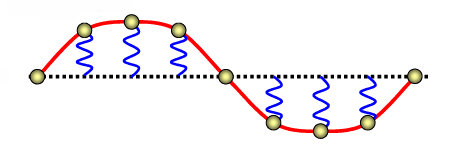
\includegraphics[width=0.8\textwidth]{Lezioni/Lezione 7/gia.png}
    \label{fig:gia}
\end{figure}
Supponiamo di avere $N$ oscillatori classici accoppiati. Ogni massa è collegata ad una molla ($k$). Le masse sono legate fra di loro da una corda senza massa che applica una tensione $\tau$
$$
L = \sum_{n=1}^N \left[ \frac{1}{2} m \dot{q}_n^2 - \frac{1}{2} k q_n^2 - \frac{1}{2} \tau \Delta x \left( \frac{q_n - q_{n-1}}{\Delta x} \right)^2 \right]
$$
Nel passaggio fa un sistema continuo
$$
m \to \rho dx \qquad q_r(t) \to \phi(x,t)
$$
$$
k \to \kappa dx \qquad \dot{q}_r(t) \to \dot{\phi}(x,t)
$$
$$
\tau \Delta x \left( \frac{q_n - q_{n-1}}{\Delta x} \right)^2 \to \tau \left( \frac{\partial \phi}{\partial x} \right)^2 dx \qquad \sum_r \to \int
$$
Pertanto la Lagrangiana diventa
$$
L = \int \left[ \frac{1}{2} \rho (\dot{\phi}(x,t))^2 - \frac{1}{2} \kappa (\phi(x,t))^2 - \frac{1}{2} \tau \left( \frac{\partial \phi}{\partial x} \right)^2 \right] dx
$$
$$
L = \int \mathcal{L} \left( \phi, \dot{\phi}, \frac{\partial \phi}{\partial x} \right) dx
$$
L'integrando è una Lagrangiana per unità di lunghezza quindi una densità di Lagrangiana. Anche nel caso continuo l'equazione di evouluzione del sistema si ottiene minimizzando l'azione
$$
S = \int L dt = \int dt dx \, \mathcal{L}(\phi, \dot{\phi}, \partial_x \phi)
$$
La condizione di minimo $\delta S=0$ conduce alle equazioni di Eulero-Lagrange
$$
\frac{\partial}{\partial t} \left( \frac{\partial \mathcal{L}}{\partial \dot{\phi}} \right) + \frac{\partial}{\partial x} \left( \frac{\partial \mathcal{L}}{\partial (\partial_x \phi)} \right) = \frac{\partial \mathcal{L}}{\partial \phi}
$$
Applichiamo questa equazioni alla desnità di Lagrangiana dell'esempio della fune
$$
\mathcal{L}(\phi, \dot{\phi}, \partial_x \phi) = \frac{1}{2}\rho\dot{\phi}^2 - \frac{1}{2}\kappa\phi^2 - \frac{1}{2}\tau(\partial_x \phi)^2
$$
$$
\frac{\partial \mathcal{L}}{\partial \dot{\phi}} = \rho\dot{\phi} \qquad \frac{\partial \mathcal{L}}{\partial (\partial_x \phi)} = -\tau \partial_x \phi \qquad \frac{\partial \mathcal{L}}{\partial \phi} = -\kappa\phi
$$
Ci conduce all'equazione del moto
$$
\rho \frac{\partial^2 \phi}{\partial t^2} - \tau \frac{\partial^2 \phi}{\partial x^2} = -\kappa\phi
$$
Abbiamo l'equazione dell'onda (sinistra) in un mezzo dispersivo (destra). Questa è l'interpretazione meccanica dell'equazione di Klein-Gordon. Il formalismo si estende facilmente al caso $3-$dimensionale
$$
\mathcal{L}(\phi, \dot{\phi}, \partial_x \phi) \to \mathcal{L}(\phi, \dot{\phi}, \nabla\phi)
$$
La densità di Lagrangiana è funzione delle $4$ derivate del campo e del campo stesso. In notazione covariante $\mathcal{L}\left(\phi,\partial_\mu\phi\right)$. Nel primo caso l'equazione di Eulero-Lagrange è
$$
\frac{\partial}{\partial t} \left( \frac{\partial \mathcal{L}}{\partial \dot{\phi}} \right) + \frac{\partial}{\partial x} \left( \frac{\partial \mathcal{L}}{\partial (\partial_x \phi)} \right) + \frac{\partial}{\partial y} \left( \frac{\partial \mathcal{L}}{\partial (\partial_y \phi)} \right) + \frac{\partial}{\partial z} \left( \frac{\partial \mathcal{L}}{\partial (\partial_z \phi)} \right) = \frac{\partial \mathcal{L}}{\partial \phi}
$$
Nel secondo caso, in notazione covariante
$$
\partial_\mu \left( \frac{\partial \mathcal{L}}{\partial (\partial_\mu \phi)} \right) = \frac{\partial \mathcal{L}}{\partial \phi}
$$
La densità è adesso per unità di volume
$$
L = \int \mathcal{L}(\phi, \partial_\mu \phi) d^3x \qquad S = \int L dt = \int \mathcal{L}(\phi, \partial_\mu \phi) d^4x
$$
Per finire, nel caso in cui il campo abbia più di una componente:
\begin{itemize}
    \item Campo di Dirac $\phi\to\psi_\sigma$ $\sigma=1,4$
    \item Campo Elettromagnetico $\phi\to A_\mu$ $\mu=0,3$
    \item Campo di Klein-Gordon complesso $\phi\to\phi_1+i\phi_2$ $\phi_1, \phi_2$ $\phi,\phi^*$
\end{itemize}
In questo caso la densità di Lagrangiana dipende da tutte le componenti
$$
\mathcal{L}(\phi_k, \partial_\mu \phi_k) \qquad k = 1,N
$$
Vale l'equazione di Eulero-Lagrange per ciascuna componente del campo
$$
\partial_\mu \left( \frac{\partial \mathcal{L}}{\partial (\partial_\mu \phi_k)} \right) = \frac{\partial \mathcal{L}}{\partial \phi_k} \qquad k = 1,N
$$
Esempio: Lagrangiana per il campo di Klein-Gordon complesso
$$
\mathcal{L}(\phi, \partial_\mu \phi, \phi^*, \partial_\mu \phi^*) = \partial_\mu \phi^* \partial^\mu \phi - m^2 \phi^* \phi
$$
$$
\frac{\partial \mathcal{L}}{\partial (\partial_\mu \phi)} = \partial^\mu \phi^* \qquad \frac{\partial \mathcal{L}}{\partial (\partial_\mu \phi^*)} = \partial^\mu \phi
$$
$$
\frac{\partial \mathcal{L}}{\partial \phi} = -m^2 \phi^*  \qquad \frac{\partial \mathcal{L}}{\partial \phi^*} = -m^2 \phi
$$
$$
\partial_\mu \partial^\mu \phi^* + m^2 \phi^* = 0 \qquad \partial_\mu \partial^\mu \phi + m^2 \phi = 0
$$
\section{Quantizzazione canonica}
Anche nel caso continuo si può utilizzare il formalismo Hamiltoniano. Dobbiamo trovare il momento coniugato della variabile dinamica. La variabile dinamica è il campo $\phi$.
$$
p = \frac{\partial L}{\partial \dot{q}} \qquad \Longrightarrow \qquad \pi = \frac{\partial \mathcal{L}}{\partial \dot{\phi}}
$$
La densità Hamiltoniana è
$$
H(p,q) = p\dot{q} - L \qquad \mathcal{H}(\pi, \phi, \partial_\mu \phi) = \pi\dot{\phi} - \mathcal{L}(\phi, \partial_\mu \phi) \qquad H = \int \mathcal{H}(\pi, \phi, \partial_\mu \phi) d^3x
$$
A questo punto si può procedere come nel caso della quantizzazione dell'oscillatore armonico unidimensionale. Si trasforma la variabile dinamica $\phi$ e il suo momento coniugato $\pi$ in operatori
$$
\phi \to \hat{\phi} \qquad \pi \to \hat{\pi} \qquad \Longrightarrow \qquad \phi(\mathbf{r}, t) \to \hat{\phi}(\mathbf{r}, t) \qquad \pi(\mathbf{r}, t) \to \hat{\pi}(\mathbf{r}, t)
$$
Osserviamo che si tratta di operatori dipendenti dal tempo. In realtà di famiglie di operatori che dipendono anche dal "parametro" $\mathbf{r}$. Si impongono regole canoniche di commutazione fra la variabile dinamica e il momento coniugato corrispondente.
$$
[\hat{q}(t), \hat{p}(t)] = i \qquad \Longrightarrow \qquad [\hat{\phi}(\mathbf{r}, t), \hat{\pi}(\mathbf{r}', t)] = i\delta^3(\mathbf{r} - \mathbf{r}')
$$
ATTENZIONE: $t$ è lo stesso per i due operatori. Poichè $\hat{\phi}(\mathbf{r},t)$ rappresenta una famiglia di operatori occorre fissare anche la regola di commutazione per i due operatori distinti $\hat{\phi}(\mathbf{r},t)$ e $\hat{\phi}(\mathbf{r}',t)$
$$
[\hat{\phi}(\mathbf{r}, t), \hat{\phi}(\mathbf{r}', t)] = 0 \qquad \text{analogamente}\qquad [\hat{\pi}(\mathbf{r}, t), \hat{\pi}(\mathbf{r}', t)] = 0
$$
Adesso vogliamo trovare una relazione per trovare $a$ e $a^\dagger$ in funzione di $\phi$ e $\pi$. Richiamiamo la rappresentazione del campo che abbiamo già utilizzato:
$$
\hat{\phi}(x) = \frac{1}{(2\pi)^3} \int \frac{d^3\mathbf{k}}{\sqrt{2k^0}} [\hat{a}_k e^{-ik\cdot x} + \hat{a}_k^\dagger e^{+ik\cdot x}]
$$
$$
k \cdot x = k^0 t - \mathbf{k} \cdot \mathbf{r} \qquad k = (k^0, \mathbf{k}) \qquad k^0 = E_k = \sqrt{\mathbf{k}^2 + m^2}
$$
Definiamo
$$
u_k(x) = \frac{e^{-ik\cdot x}}{\sqrt{(2\pi)^3 2k^0}} \qquad f_1 \overleftrightarrow{\partial}_\mu f_2 = f_1 (\partial_\mu f_2) - (\partial_\mu f_1) f_2
$$
Le funzioni $u_k(x)$ soddisfano le relazioni di ortogonalità standard
$$
\int u_k^*(x) u_{k'}(x) \frac{d^3\mathbf{r}}{(2\pi)^3} = \frac{1}{2k^0} \delta(\mathbf{k} - \mathbf{k}')
$$
Da notare che non dipendono dal tempo $t$. Inoltre, soddisfano le seguenti ulteriori regole di ortogonalità generalizzata 
$$
\int u_k^*(x) i \overleftrightarrow{\partial}_0 u_{k'}(x) \frac{d^3\mathbf{r}}{(2\pi)^3} = \delta(\mathbf{k} - \mathbf{k}') \qquad \int u_k(x) i \overleftrightarrow{\partial}_0 u_{k'}^*(x) \frac{d^3\mathbf{r}}{(2\pi)^3} = -\delta(\mathbf{k} - \mathbf{k}')
$$
$$
\int u_k(x) i \overleftrightarrow{\partial}_0 u_{k'}(x) \frac{d^3\mathbf{r}}{(2\pi)^3} = 0 \qquad \int u_k^*(x) i \overleftrightarrow{\partial}_0 u_{k'}^*(x) \frac{d^3\mathbf{r}}{(2\pi)^3} = 0
$$
Si può verificare che valgono le seguenti relazioni
$$
\hat{a}_p = \int u_p^*(x) (p^0 \hat{\phi}(x) + i \hat{\pi}(x)) d^3\mathbf{r} \qquad \hat{a}_p = \int u_p^*(x) i \overleftrightarrow{\partial}_0 \hat{\phi}(x) d^3\mathbf{r}
$$
$$
\hat{a}_p^\dagger = \int u_p(x) (p^0 \hat{\phi}(x) - i \hat{\pi}(x)) d^3\mathbf{r} \qquad \hat{a}_p^\dagger = - \int u_p(x) i \overleftrightarrow{\partial}_0 \hat{\phi}^\dagger(x) d^3\mathbf{r}
$$
Calcoliamo il commutatore
$$
[\hat{a}_k, \hat{a}_p^\dagger] = \int d^3\mathbf{r} d^3\mathbf{r}' u_k^*(x) u_p(x') \{ [k^0 \hat{\phi}(x) + i \hat{\pi}(x)], [p^0 \hat{\phi}(x') - i \hat{\pi}(x')] \}
$$
Elaboriamo l'integrando ricordando che
$$
[\hat{\phi}(\mathbf{r}, t), \hat{\pi}(\mathbf{r}', t)] = i\delta^3(\mathbf{r} - \mathbf{r}')
$$
$$
[,] = u_k^*(x) u_p(x') \{ -i k^0 \hat{\phi}(x) \hat{\pi}(x') + i \hat{\pi}(x) p^0 \hat{\phi}(x') \}
$$$$
[,] = u_k^*(x) u_p(x') \{ -i i k^0 \delta(\mathbf{r} - \mathbf{r}') - i i p^0 \delta(\mathbf{r} - \mathbf{r}') \}
$$
Introducendo nell'integrale
$$
[\hat{a}_k, \hat{a}_p^\dagger] = \int d^3\mathbf{r} d^3\mathbf{r}' u_k^*(x) u_p(x') \{ k^0 \delta(\mathbf{r} - \mathbf{r}') + p^0 \delta(\mathbf{r} - \mathbf{r}') \}
$$
Ricordiamo
$$
\int u_k^*(x) u_{k'}(x) \frac{d^3\mathbf{r}}{(2\pi)^3} = \frac{1}{2k^0} \delta(\mathbf{k} - \mathbf{k}')
$$
$$
[\hat{a}_k, \hat{a}_p^\dagger] = \int d^3\mathbf{r} \{ (k^0 u_k^*(x) u_p(x) + p^0 u_k^*(x) u_p(x) \}
$$
$$
[\hat{a}_k, \hat{a}_p^\dagger] = \frac{(2\pi)^3}{2k^0} \{ k^0 \delta(\mathbf{k} - \mathbf{p}) + p^0 \delta(\mathbf{k} - \mathbf{p}) \} = (2\pi)^3 \delta(\mathbf{k} - \mathbf{p})
$$
\subsection{Calcolo dell'Hamiltoniano}
Calcoliamo l'Hamiltoniano in funzione degli operatori di creazione e distruzione per il campo di Klein-Gordon reale. Utilizzando il formalismo Hamitloniano
$$
\mathcal{H}(\pi, \phi, \partial_\mu \phi) = \pi\dot{\phi} - \mathcal{L}(\phi, \partial_\mu \phi) \qquad \mathcal{L} = \frac{1}{2}[\partial^\mu \phi \partial_\mu \phi - m^2 \phi^2] \qquad \hat{H} = \int \mathcal{H} d^3\mathbf{r}
$$
$$
\mathcal{H} = \dot{\phi}\dot{\phi} - \frac{1}{2}\partial^\mu \phi \partial_\mu \phi + \frac{1}{2}m^2 \phi^2 = \frac{1}{2}[\dot{\phi}\dot{\phi} + \boldsymbol{\nabla}\phi \cdot \boldsymbol{\nabla}\phi + m^2\phi^2] \qquad\pi = \frac{\partial \mathcal{L}}{\partial \dot{\phi}} = \dot{\phi}
$$
$$
\hat{H} = \frac{1}{2} \int [\hat{\dot{\phi}}\hat{\dot{\phi}} + \boldsymbol{\nabla}\hat{\phi} \cdot \boldsymbol{\nabla}\hat{\phi} + m^2\hat{\phi}^2] d^3\mathbf{r}
$$
A questo punto, si potrebbero inserire le espansioni dei campi e utlimare il calcolo in modo analogo a quanto fatto per il campo elettromagnetico
$$
\hat{\phi}(x) = \frac{1}{(2\pi)^3} \int \frac{d^3\mathbf{k}}{\sqrt{2\omega}} [\hat{a}_k e^{-ik\cdot x} + \hat{a}_k^\dagger e^{+ik\cdot x}]
$$
$$
\boldsymbol{\nabla}\hat{\phi}(x) = \frac{1}{(2\pi)^3} \int \frac{d^3\mathbf{k}}{\sqrt{2\omega}} i\mathbf{k} [\hat{a}_k e^{-ik\cdot x} - \hat{a}_k^\dagger e^{+ik\cdot x}]
$$
$$
\dot{\hat{\phi}}(x) = \frac{1}{(2\pi)^3} \int \frac{d^3\mathbf{k}}{\sqrt{2\omega}} (-i\omega) [\hat{a}_k e^{-ik\cdot x} - \hat{a}_k^\dagger e^{+ik\cdot x}]
$$
Dopo vari conti che non riporto 
$$
\hat{H} = \frac{1}{(2\pi)^3} \int d^3\mathbf{k} E_k \frac{1}{2} [\hat{a}_k \hat{a}_k^\dagger + \hat{a}_k^\dagger \hat{a}_k]
$$
Notiamo che l'espressione trovata è indipendente dal tempo. Le regole di ortogonalità delle funzioni $u_k$ rimuovono la dipendenza da $t$. Il risultato che abbiao trovato è molto simile a quanto avevamo trovato intuitivamente. Trasformiamo ulteriormente l'espressione trovata usando le regole di commutazione degli operatori di creazione e distruzione
$$
[\hat{a}_k, \hat{a}_k^\dagger] = 1 \to \hat{a}_k \hat{a}_k^\dagger = 1 + \hat{a}_k^\dagger \hat{a}_k
$$
$$
\hat{H} = \frac{1}{(2\pi)^3} \int d^3k E_k \left[ \hat{a}_k^\dagger \hat{a}_k + \frac{1}{2} \right]
$$
L'Hamiltoniano è la somma delle energie dei singoli oscillatori. Il termine $\frac{1}{2}E_k$ è legato all'energia del vuoto nell'oscillatore. Nel caso di un campo porta ad un contributo divergente. Viene eliminato imponendo che i campi abbiamo un ordinamento normale. In un prodotto normale $\left(:AB:\right)$ gli operatori di distruzione stanno a destra.
\section{Teorema di Noether}
Noether era una signora, è importante dirlo perché quando era uscito questo lavoro nessuno lo ha citato ma lo usavano tutti. Abbiamo già visto che le equazioni di campo si deducono minimizzando l'azione (quindi imponendo la variazione dell'azione uguale a zero) portandoci all'equazione di Eulero-Lagrange
$$
S = \int \mathcal{L}(\phi, \partial_\mu \phi) d^4x \qquad \delta S = 0 \quad \Longrightarrow \quad \partial_\mu \left( \frac{\partial \mathcal{L}}{\partial (\partial_\mu \phi)} \right) = \frac{\partial \mathcal{L}}{\partial \phi}
$$
Il teorema di Noether permette di derivare le leggi di conservazione dalle proprietà di simmetria dell'azione (e quindi della Lagrangiana). L'azione può essere lasciata invariata da vari tipi di trasformazioni:
\begin{itemize}
    \item di simmetria interna. Con questa intendo (di solito si applica quando ci sono più gradi di libertà e componenti) qualcosa che mi mescola le componenti ma mi lascia invariata la densità di Lagrangiana (ad esempio isospin, gauge)
    \item di simmetria spazio-temporale (trasformazioni di Lorentz + traslazioni)
\end{itemize}
Il teorema di Noether asserisce che ad ogni simmetria differenziabile (importantissimo e fondamentale perché significa che la simmetria dipende da parametri e questa dipendenza è di tipo continuo. Ad esempio la simmetria di parità non è differenziabile!) che lascia invariata l'azione corrisponde una corrente conservata e, di conseguenza, una carica conservata. Dato che l'azione è un integrale su $d^4x$ la trasformazione di simmetria deve lasciare invariata la lagrangiana $\delta\mathcal{L}=0$. Al più variare la lagrangiana di una $4-$divergenza ($\delta\mathcal{L}=\partial_\mu f^\mu$) che per il teorema di Gauss $4-$dimensionale non contribuisce all'azione
$$
\int \partial_\mu j^\mu d^4x = \oint j^\mu dS_\mu \to 0
$$
Tipicamente, per le simmetrie interne il termine di $4-$divergenza è nullo. Invece questa non è nulla nel caso di simmetria dello spazio-tempo (trasformazioni del gruppo di Poincaré: Trasformazioni di Lorentz e traslazioni). L'applicazione di una trasformazione del gruppo di simmetria provoca una variazione dei campi $\phi\to\phi+\delta\phi$. La variazione dei campi induce una variazione della Lagrangiana $\mathcal{L}\to\mathcal{L}+\delta\mathcal{L}$. Nel caso delle simmetrie interne $\delta\mathcal{L}=0$ quindi esiste una corrente $j^\mu$ conservata $\partial_\mu j^\mu=0$. Nel caso di simmetrie dello spazio-tempo $\delta\mathcal{L}=\partial_\mu f^\mu$ esiste una corrente $j^\mu$ tale che $\partial_\mu j^\mu=\partial_\mu f^\mu \to \partial_\mu(j^\mu-f^\mu)=0$. La corrente conservata implica l'esistenza di una carica conservata.
$$
\frac{\partial \rho}{\partial t} = \boldsymbol{\nabla} \cdot \mathbf{j} \qquad \Longrightarrow \qquad \int_V \frac{\partial \rho}{\partial t} dV = \int_V \boldsymbol{\nabla} \cdot \mathbf{j} dV = \oint_S \mathbf{j} \cdot d\mathbf{a} = 0
$$
$$
Q = \int \rho dV \qquad \frac{\partial Q}{\partial t} = 0
$$
Per campi che vanno a zero all'infinito rapidamente.
\begin{figure}[h!]
    \centering
    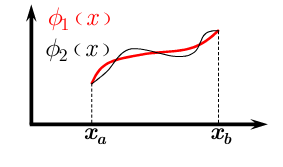
\includegraphics[width=0.7\textwidth]{Lezioni/Lezione 7/ku.png}
    \label{fig:ku}
\end{figure}
Una variazione $\delta\phi(x)$ di un campo è una funzione infinitesima e che si annulla agli estremi
$$
\delta\phi(x) = \phi_1(x) - \phi_2(x) \qquad \delta\phi(x_a) = \delta\phi(x_b) = 0
$$
L'operazione di variazione commuta con la derivazione. L'espressione $\partial_\mu\phi$ è una funzione (che dipende da $\phi$)
$$
\delta[\partial_\mu\phi(x)] = \partial_\mu\phi_1(x) - \partial_\mu\phi_2(x) = \partial_\mu[\phi_1(x) - \phi_2(x)] = \partial_\mu\delta\phi(x)
$$
Veniamo ora alla dimostrazione del teorema. Per generalità supponiamo che la lagrangiana dipenda da più campi $(n=1,N)$
$$
\mathcal{L} = \mathcal{L}(\phi_n, \partial_\mu\phi_n)
$$
Calcoliamo la variazione della Lagrangiana
$$
\delta\mathcal{L} = \mathcal{L}(\phi_n + \delta\phi_n, \partial_\mu\phi_n + \delta\partial_\mu\phi_n) - \mathcal{L} \approx \sum_{n=1}^N \left[ \frac{\partial\mathcal{L}}{\partial\phi_n}\delta\phi_n + \frac{\partial\mathcal{L}}{\partial(\partial_\mu\phi_n)}\delta\partial_\mu\phi_n \right]
$$
Elaboriamo l'espressione commutando $\delta$ con $\partial_\mu$ nel secondo termine e utilizzando l'equazione di Eulero-Lagrange nel primo
$$
\partial_\mu \frac{\partial\mathcal{L}}{\partial(\partial_\mu\phi_n)} = \frac{\partial\mathcal{L}}{\partial\phi_n}
$$
$$
\delta\mathcal{L} = \sum_{n=1}^N \partial_\mu \left( \frac{\partial\mathcal{L}}{\partial(\partial_\mu\phi_n)} \right) \delta\phi_n + \frac{\partial\mathcal{L}}{\partial(\partial_\mu\phi_n)}\partial_\mu\delta\phi_n
$$
L'espressione può essere trasformata in una $4-$divergenza
$$
\delta\mathcal{L} = \partial_\mu \sum_n \frac{\partial\mathcal{L}}{\partial(\partial_\mu\phi_n)}\delta\phi_n
$$
Se la trasformazione di simmetria modifica solo i campi ma lascia invariata la lagrangiana allora la variazione è nulla: $\delta\mathcal{L}=0$. Otteniamo pertanto
$$
\partial_\mu \sum_n \frac{\partial\mathcal{L}}{\partial(\partial_\mu\phi_n)}\delta\phi_n = 0
$$
Abbiamo inoltre supposto che l'operazione di simmetria sia differenziabile. In generale, la variazione del campo dipende da $M$ parametri arbitrari (ad esempio, una rotazione dipende da $3$ parametri)
$$
\delta\phi_n = \sum_{k=1}^M \frac{\delta\phi_n}{\delta\varepsilon^k} \delta\varepsilon^k
$$
Poichè la variazione dei campi è arbitraria possiamo variare gli $M$ parametri indipendentemente (uno a uno) e otteniamo $M$ espressioni
$$
\partial_\mu \sum_n \frac{\partial\mathcal{L}}{\partial(\partial_\mu\phi_n)} \frac{\delta\phi_n}{\delta\varepsilon^k} = 0 \qquad k = 1,M
$$
Possiamo pertanto definire le $M$ correnti conservate
$$
j^{k,\mu} = \sum_n \frac{\partial\mathcal{L}}{\partial(\partial_\mu\phi_n)} \frac{\delta\phi_n}{\delta\epsilon^k} \qquad k = 1,M \qquad \partial_\mu j^{k,\mu} = 0
$$
La natura dell'indice $k$ dipende dal tipo di trasformazione. Può essere un indice di Lorentz. In questo caso la corrente è un tensore. O può essere un indice che individua un grado di libertà interno ad esempio l'isospin. Illustriamo i concetti introdotti con due esempi: un esempio di simmetria dello spazio-tempo (le traslazioni) e un esempio di simmetria interna (trasformazione di gauge).